\documentclass[pdf, 10pt, unicode]{beamer}

\usepackage[T2A]{fontenc}
%\usepackage[cp1251]{inputenc}
\usepackage[utf8]{inputenc}
\usepackage[russian,english]{babel}
\usepackage{minted}
\usemintedstyle{perldoc}
\usepackage{graphicx}
\usepackage{amssymb}
\usepackage{amsthm}
\usepackage{amsmath}
\usepackage{tabularx}
\usepackage{multicol}
\usepackage{multirow}
\usepackage{calrsfs}
\usepackage{listings}
\usepackage{color}

\usepackage{array}
\newcolumntype{L}[1]{>{\raggedright\let\newline\\\arraybackslash\hspace{0pt}}m{#1}}
\newcolumntype{C}[1]{>{\centering\let\newline\\\arraybackslash\hspace{0pt}}m{#1}}
\newcolumntype{R}[1]{>{\raggedleft\let\newline\\\arraybackslash\hspace{0pt}}m{#1}}

% \lstset{basicstyle=\fontsize{7pt}{1em}\ttfamily,
%         keywordstyle=\fontsize{7pt}{1em}\color{MOOCBlue}\bfseries,
%         commentstyle=\fontsize{7pt}{1em}\ttfamily\color{MOOCGreen}}


\usepackage{caption}
\usepackage{subcaption}

% \lstset{language=C++,
%   basicstyle=\footnotesize\itshape,
%   keywordstyle=\color{black}\bfseries\underbar,
%   % underlined bold black keywords
%   identifierstyle={\color{black}},%
%   commentstyle=\color{brown}, % brown comments
%   stringstyle=\color{blue}\ttfamily, % typewriter type for strings, blue
%   showstringspaces=false
% }

\definecolor{MOOCGrey}{RGB}{230,230,230}
\definecolor{MOOCBlue}{RGB}{38,57,200}
\definecolor{MOOCGreen}{RGB}{38,130,63}

\lstset{extendedchars=true}
\lstset{language=C++, basicstyle=\small\ttfamily,  keywordstyle=\small\color{MOOCBlue}\bfseries,
        commentstyle=\small\ttfamily\color{MOOCGreen}, showstringspaces=false,
        extendedchars=true, texcl=true, frame=single,
        morekeywords={size_t}}



\newenvironment{changemargin}[2]{%
\begin{list}{}{%
\setlength{\topsep}{0pt}%
\setlength{\leftmargin}{#1}%
\setlength{\rightmargin}{#2}%
\setlength{\listparindent}{\parindent}%
\setlength{\itemindent}{\parindent}%
\setlength{\parsep}{\parskip}%
}%
\item[]}{\end{list}}


\usetheme{Copenhagen}
\usepackage{color}

\usecolortheme[RGB={50,100,200}]{structure}

\setbeamertemplate{navigation symbols}{}
\setbeamertemplate{itemize
item}{\scriptsize\raise1.25pt\hbox{\donotcoloroutermaths$\blacktriangleright$}}

\setbeamertemplate{frametitle continuation}[from second]

\title{stdio окончание. heap. ДЗ (указатели на функции, список).}
\author{Евгений Линский}
\date{}
\usefonttheme[onlymath]{serif}

\setbeamerfont{institute}{size=\normalsize}

\setbeamertemplate{footline} {
  \hbox{%
  \begin{beamercolorbox}[wd=0.08\paperwidth,ht=2.5ex,dp=0ex,left]{title in head/foot}%
  \end{beamercolorbox}%
  \begin{beamercolorbox}[wd=0.46\paperwidth,ht=2.5ex,dp=1ex,center]{title in head/foot}%
    \usebeamerfont{title in head/foot}{C++}%\insertshortauthor %\insertshorttitle
  \end{beamercolorbox}%
  \begin{beamercolorbox}[wd=0.46\paperwidth,ht=2.5ex,dp=1ex,right]{date in head/foot}%
    \usebeamerfont{date in head/foot}
    \insertframenumber{} / \inserttotalframenumber{}\hspace*{2ex}
  \end{beamercolorbox}}%
  \vskip0pt%
}

\sloppy

\begin{document}
\begin{frame}
  \vspace{1cm}
  \large
  \maketitle
  \thispagestyle{empty}
  \vspace{1cm}
  \date{}
\end{frame}

\begin{frame}[fragile]{{\tt stdio}}
\begin{center}
\begin{huge}stdio окончание\end{huge}
\end{center}
\end{frame}


\begin{frame}[fragile]{{\tt printf/fprintf/sprintf}}
\begin{lstlisting}
fprintf(stdout, ...); //printf
fscanf(stdin, ....); //scanf
char s1[] = "3  4";
sscanf(s1,"%d %d", &a, &b);
char s2[256];
sprintf(s2, "%d + %d = %d", a, b, c);
\end{lstlisting}
\begin{enumerate}
  \item Все это небыстро, т.к. внутри функции нужно разобрать форматную строку
  \item Технология: функция с переменным числом параметров (см. \emph{va\_arg})
\end{enumerate}
\url{https://en.cppreference.com/w/cpp/io/c/fprintf}
\end{frame}


\begin{frame}[fragile]{{\tt Переменное число аргументов в C (printf)}}
va\_start, va\_arg, va\_end --- макросы.
\begin{minted}[linenos=true]{cpp}
void simple_printf(const char* fmt, ...) {
  va_list args;
  //записать в args адрес следующего за fmt параметра на стеке
  va_start(args, fmt);
  while(*fmt != '\0') {
    if(*fmt=='d') {
      //достать со стека переменную типа int
      int i = va_arg(args, int)
      // здесь должен быть код, который
      // выводит int на экран с помощью putc
    }
    fmt++;
  }
  va_end(args);
}
//Труднообнаруживаемые ошибки
printf("%s", 5);
printf("%d %d", 4); printf("%d", 4, 5);
\end{minted}

\end{frame}

\begin{frame}[fragile]{{\tt Heap}}
\begin{center}
\begin{huge}Куча\end{huge}
\end{center}
\end{frame}

\begin{frame}[fragile]{{\tt Три вида памяти в программе на C}}

\begin{enumerate}
  \item \textbf{Стек} (stack)
    \begin{itemize}
        \item локальные переменные функций, параметры функций
        \item код для выделения и освобождения генерирует компилятор
        \item выделяется при ``входе'' в функцию, освобождается при ``выходе'' из функции
    \end{itemize}
  \item \textbf{Глобальная память} (static variables)
    \begin{itemize}
        \item глобальные переменные (вне функций), статические переменные (static)
        \item код для выделения и освобождения генерирует компилятор
        \item выделяется при загрузке в память, освобождается при завершении программы
        \item глобальные инициализируются в \textit{каком-то} порядке,
              статические~--- при входе в функцию
    \end{itemize}

  \item \textbf{Куча} (heap)
    \begin{itemize}
        \item код для выделения и освобождения пишет программист
    \end{itemize}

\end{enumerate}

\end{frame}

\begin{frame}[fragile]{{\tt Карта памяти}}
\begin{itemize}
  \item Расположение частей может отличаться на разных платформах.
  \item В общем случае адресация неважна.
  \item Ниже один из вариантов (``упрощенный linux'', 4 Gb)
\end{itemize}

\begin{tabular}{|l|}
\hline
OS kernel (например, 1 Gb)\\
$\ldots$.\\
\hline
Stack, растет вниз \textdownarrow (например, 10 Mb)\\
\hline
$\ldots$.\\
$\ldots$.\\
$\ldots$.\\
Heap, растет вверх \textuparrow (например, $\sim$2,9 Gb)\\
\hline
Static variables (например, 10 Mb)\\
\hline
Двоичный код программы (например, 10 Mb)\\
\hline
\end{tabular}

\end{frame}


\begin{frame}[fragile]{{\tt Куча. }}
\begin{minted}[linenos=true]{cpp}
#include <stdlib.h>

int *p = malloc(1000000 * sizeof(int));
if (p == NULL){  // NULL в C, nullptr в C++. Старый код - 0.
  /* not enough memory */
}
// if (!p) { ... } // Альтернативный вариант
p[0] = 1; p[13000]  = 42;
...
free(p);

\end{minted}

\begin{enumerate}
  \item Временем жизни управляет программист
  \item \emph{Функция} malloc обращается к операционной системе с просьбой (sbrk) выделить место (``непрерывный кусок'') в куче и, если ОС выделяет это место, возвращает укзатель на начало области (иначе --- 0).
  \item \emph{Функция} free освобождает память
  \item Нет ограничений по размеру как у стека и глобальных переменных (ограничена размером свободной памяти)
\end{enumerate}

\end{frame}

\begin{frame}[fragile]{{\tt Куча. }}
\begin{minted}[linenos=true]{cpp}
#include <stdlib.h>
#include <stdio.h>

size_t size = 0;
// %zu вместо %d, потому что size_t может != int.
scanf("%zu", &size);
int *array = malloc(size * sizeof(int));
\end{minted}

\begin{enumerate}
  \item Размер массива выясняется во время выполнения (ввел пользователь, считали из файла)
  \item На стеке и у глобальных переменных размер должен быть известен во время компиляции
\end{enumerate}

\end{frame}

\begin{frame}[fragile]{{\tt Куча. Ошибки.}}

\begin{minted}[linenos=true]{cpp}
int *p = malloc(sizeof(int));
free(p);
\end{minted}
Что не так?
\begin{enumerate}
\uncover<2->{\item Занимает в три раза больше места чем на стеке (int*, int)}
\end{enumerate}

\end{frame}

\begin{frame}[fragile]{{\tt Куча. Ошибки.}}
\begin{minted}[linenos=true]{cpp}
int *p = (int *)malloc(1000000 * sizeof(int));
p = (int *)malloc(1000000 * sizeof(int));
// Или: p = NULL;
\end{minted}
\begin{itemize}
  \item Утечка памяти (memory leak): теперь память из первой строки невозможно освободить (мы потеряли адрес)
  \item Такие ошибки можно искать утилитой \emph{valgrind}
\end{itemize}
Вопрос! В современных ОС вся память, выделенная программой, после ее завершения возвращается системе (даже если была утечка). Зачем бороться с утечками?
\begin{enumerate}
\uncover<2->{\item Сервер (работает без перезапуска). Утечка при каждом запросе пользователя.}
\uncover<3->{\item Сначала все замедлится (файл подкачки), потом ОС аварийно завершит процесс.}
\end{enumerate}

\end{frame}

\begin{frame}[fragile]{{\tt Куча. Вычислительная сложность}}
malloc должен:
\begin{enumerate}
    \item Пройти по списку (одна из возможным реализаций) выделенных (точнее <<выделенных, но потом освобожденных>>, см. дз alloc) областей
    \item Найти непрерывную область нужного размера
\end{enumerate}
Это гораздо дольше чем на стеке и у глобальных переменных!
\end{frame}

\begin{frame}[fragile]{{\tt Куча. Что еще бывает?}}
\begin{itemize}
  \item calloc --- выделяет память и инициализирует ее нулями
  \item realloc --- изменяет размер уже существующего массива. Существует три результата работы функции:
  \begin{enumerate}
    \item если нужное число байт не занято в данной области памяти, то увеличивает область для массива
    \item если рядом нет свободной памяти, перенесет массив в другое место
    \item если вообще нет памяти под увеличенный массив, вернет 0
  \end{enumerate}
\end{itemize}
\end{frame}

\begin{frame}[fragile]{{\tt ДЗ}}
\begin{center}
\begin{huge}ДЗ\end{huge}
\end{center}
\end{frame}


\begin{frame}[fragile]{{\tt binary-search-3: сортировка выбором}}
Рассмотрим на примере более простой сортировки.\\
selection\_sort
  \begin{lstlisting}
void sel_sort(int *arr, int n) {
    int i, j, min_idx;

    for (i = 0; i < n-1; i++) {
        min_idx = i;
        for (j = i + 1; j < n; j++)
          if (arr[j] < arr[min_idx])
            min_idx = j;
        swap(&arr[min_idx], &arr[i]);
    }
}

  \end{lstlisting}

\end{frame}

\begin{frame}[fragile]{{\tt Любой тип данных: void*.}}
\begin{lstlisting}
struct product_s {
  char label[256];
  unsigned char weight;
  unsigned int price;
};
typedef struct product_s product_t;
\end{lstlisting}

\begin{lstlisting}
void sel_sort(void *array, size_t n, ...);

product_t array1[100];
int arrray2[20];
sel_sort(array1, 100, ...);
sel_sort(array2, 20, ...)
\end{lstlisting}

\begin{itemize}
  \item void* --- не работает адресная арифметика
  \item В С++ неявное приведение типа в void* не вызывает ошибки (в С все можно неявно)
  \item В С++ требуется явное приведение типа из void* (в С все можно неявно)
  \item void* malloc(...)
\end{itemize}

\end{frame}

\begin{frame}[fragile]{{\tt Переставлять любые элементы: swap.}}
\begin{lstlisting}
void sel_sort(void *array, size_t n, size_t elem_size, ...) {
  char *p = array;
  //смысл: swap(\&array[i], \&array[j])
  swap(p + i * elem_size, p + j * elem_size, elem_size);
}
void swap(char *p1, char *p2, size_t elem_size) {
  int i = 0; char tmp = 0;
  while( i < elem_size ) {
    tmp = *(p1 + i);
    *(p1 + i) = *(p2 + i);
    *(p2 + i) = tmp;
    i++;
  }
}
\end{lstlisting}
\end{frame}

\begin{frame}[fragile]{{\tt Сравнивать любые элементы: cmp.}}
Указатель --- адрес в памяти:
\begin{itemize}
  \item В памяти хранятся переменные и двоичный код (двоичные инструкции нашей программы)
  \item Можно хранить адрес переменной (указатель)
  \item Можно хранить адрес кода (указатль на функцию)
\end{itemize}
\begin{lstlisting}
void dummy(int x) {
    printf( "%d\n", x );
}

int main() {
  void (*func)(int);
  func = &dummy;
  (*func)(2);
  // можно и так:
  func = dummy;
  func(2);
  return 0;
}
\end{lstlisting}
\end{frame}

\begin{frame}[fragile]{{\tt Сравнивать любые элементы: cmp.}}
\begin{lstlisting}
void sel_sort(void *array, size_t size, size_t elem_size,
            int (*cmp)(void *p1, void *p2)) {
  char *p = array;
  //смысл: if (array[i] < array[j])
  if (cmp(p + i * elem_size, p + j * elem_size))

}
int cmp_int(void *p1, void *p2) {
  int *pi1 = p1; int *pi2 = p2;
  return (*pi1 - *pi2);
}
int cmp_product_by_weight(void *p1, void *p2) {
  product_t *pp1 = p1; product_t *pp2 = p2;
  return (*pp1->weight- *pp2->weight);
}
product_t array1[100];
int arrray2[20];
sel_sort(array1, 100, sizeof(array1[0]),
  cmp_product_by_weight);
sel_sort(array2, 20, sizeof(array2[0]), cmp_int);
\end{lstlisting}

\end{frame}


\begin{frame}[fragile]{{\tt alloc: связный список}}

\begin{itemize}
  \item размер может увеличиваться при добавлении элементов
    \begin{itemize}
        \item каждый элемент выделяется с помощью malloc
        \item элементы расположены на произвольных (в векторе --- на последовательных) адресах
        \item каждый элемент хранит адреса следующего и предыдущего (необязательно)
    \end{itemize}
    \item из-за того, что адреса элементов непоследовательные, не требуется смещать элементы при этих операциях вставки и удаления

\end{itemize}

\end{frame}

\begin{frame}[fragile]{{\tt list}}
    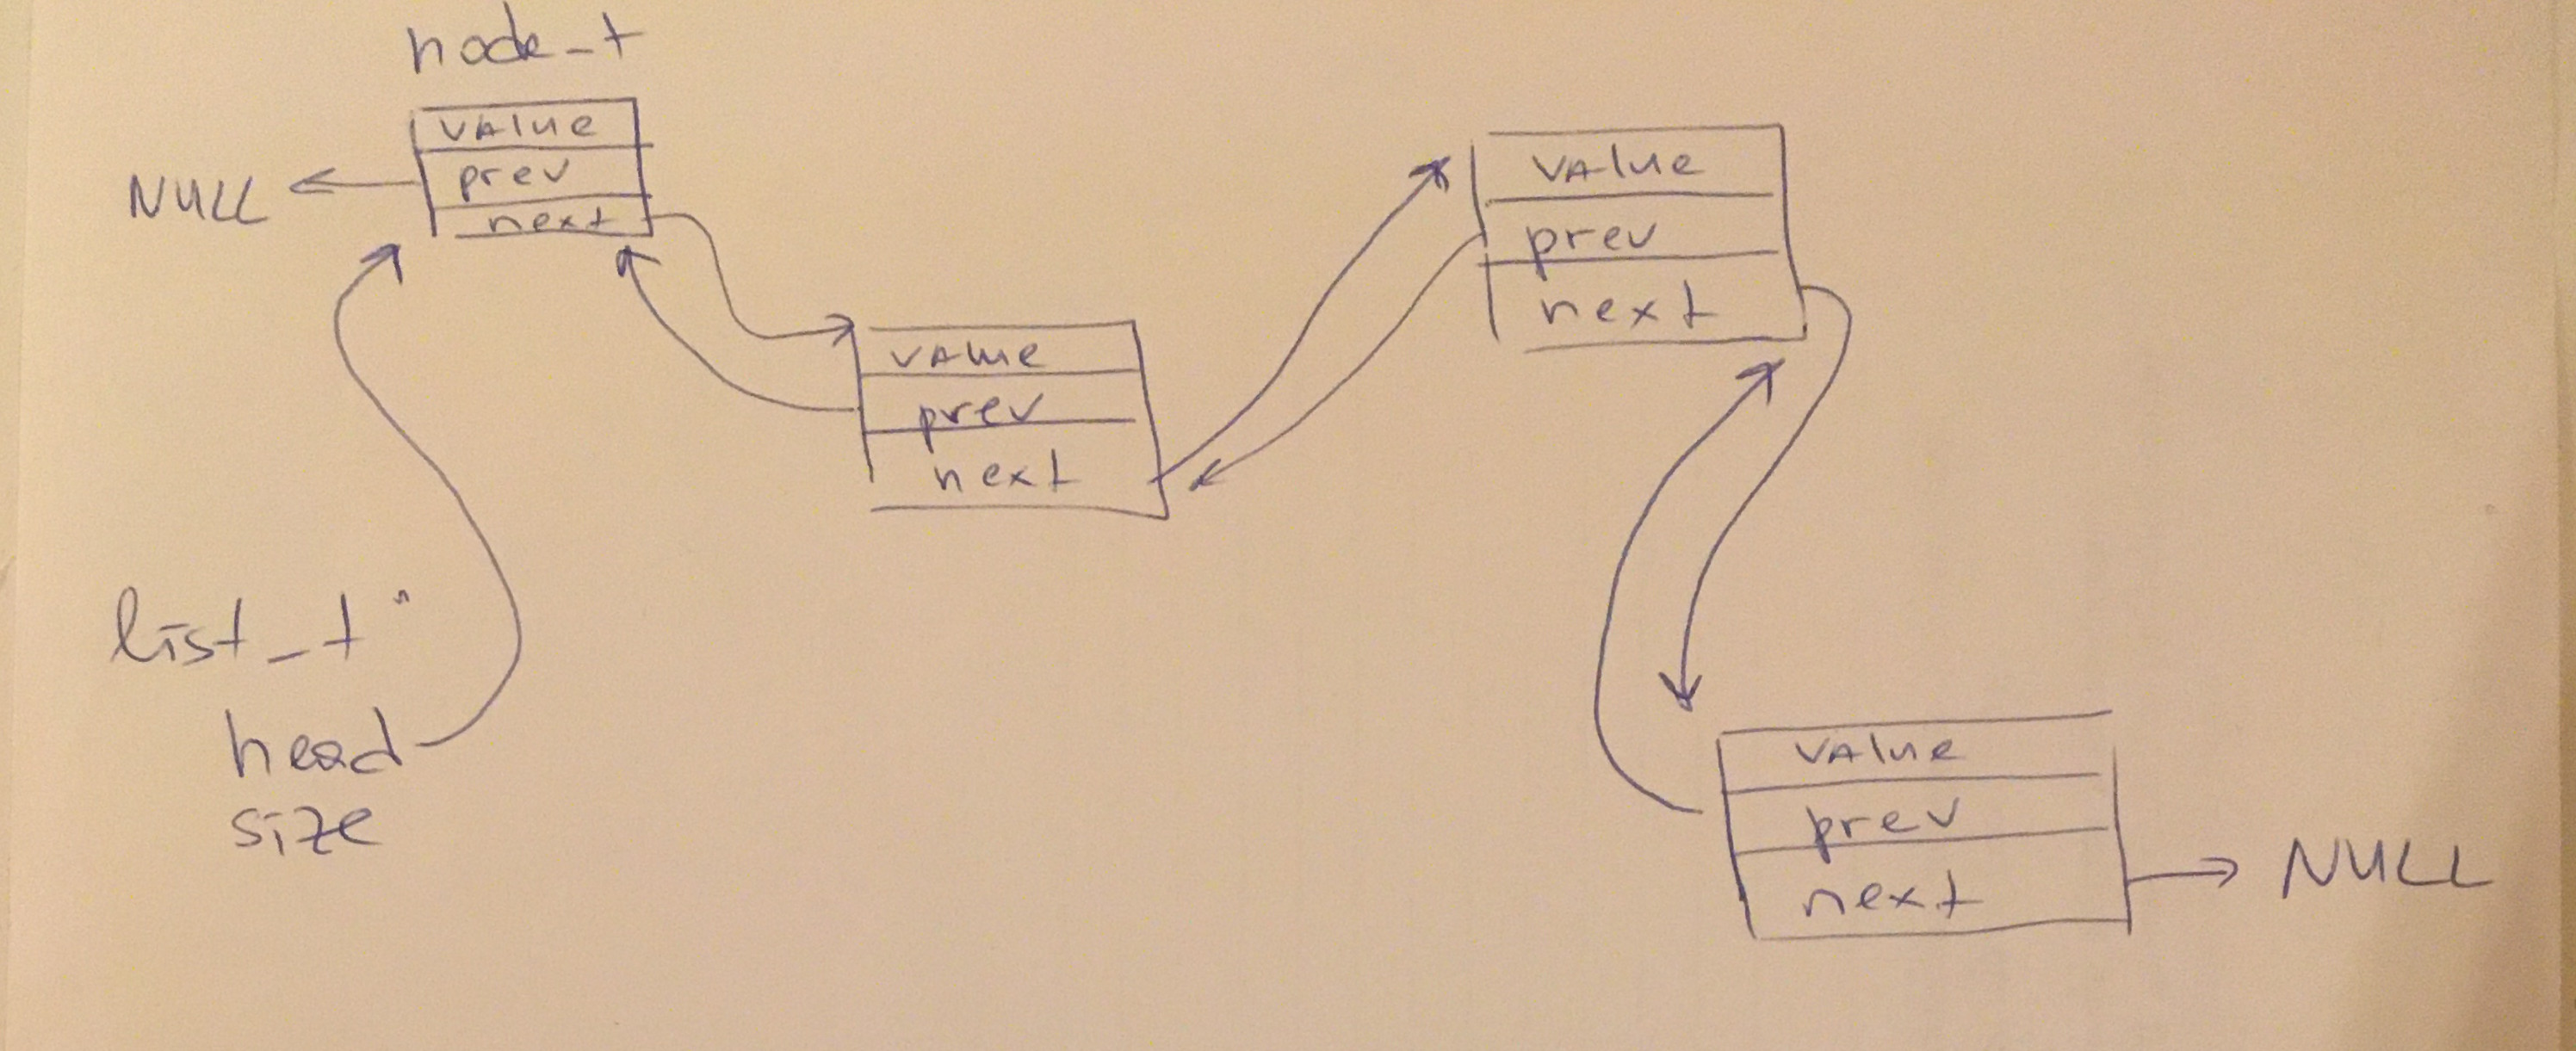
\includegraphics[scale=0.1]{list_in_mem}
\end{frame}

\begin{frame}[fragile]{{\tt node\_t}}
\begin{lstlisting}
struct node_s; // forward declaration

typedef struct node_s {
  int value;
  struct node_s *prev; // адрес предыдущего (необязательно)
  struct node_s *next; // адрес следующего
} node_t;

node_t *head = NULL; // адрес нулевого элемента
\end{lstlisting}
\end{frame}

\begin{frame}[fragile]{{\tt print}}
\begin{lstlisting}
void print(node_t *head) {
  node_t *cur = head;
  while (cur != NULL) {
    printf("%d ", cur->value);
    cur = cur->next;
  }
  printf("\n");
}
\end{lstlisting}
\end{frame}

\begin{frame}[fragile]{{\tt list iterate}}
    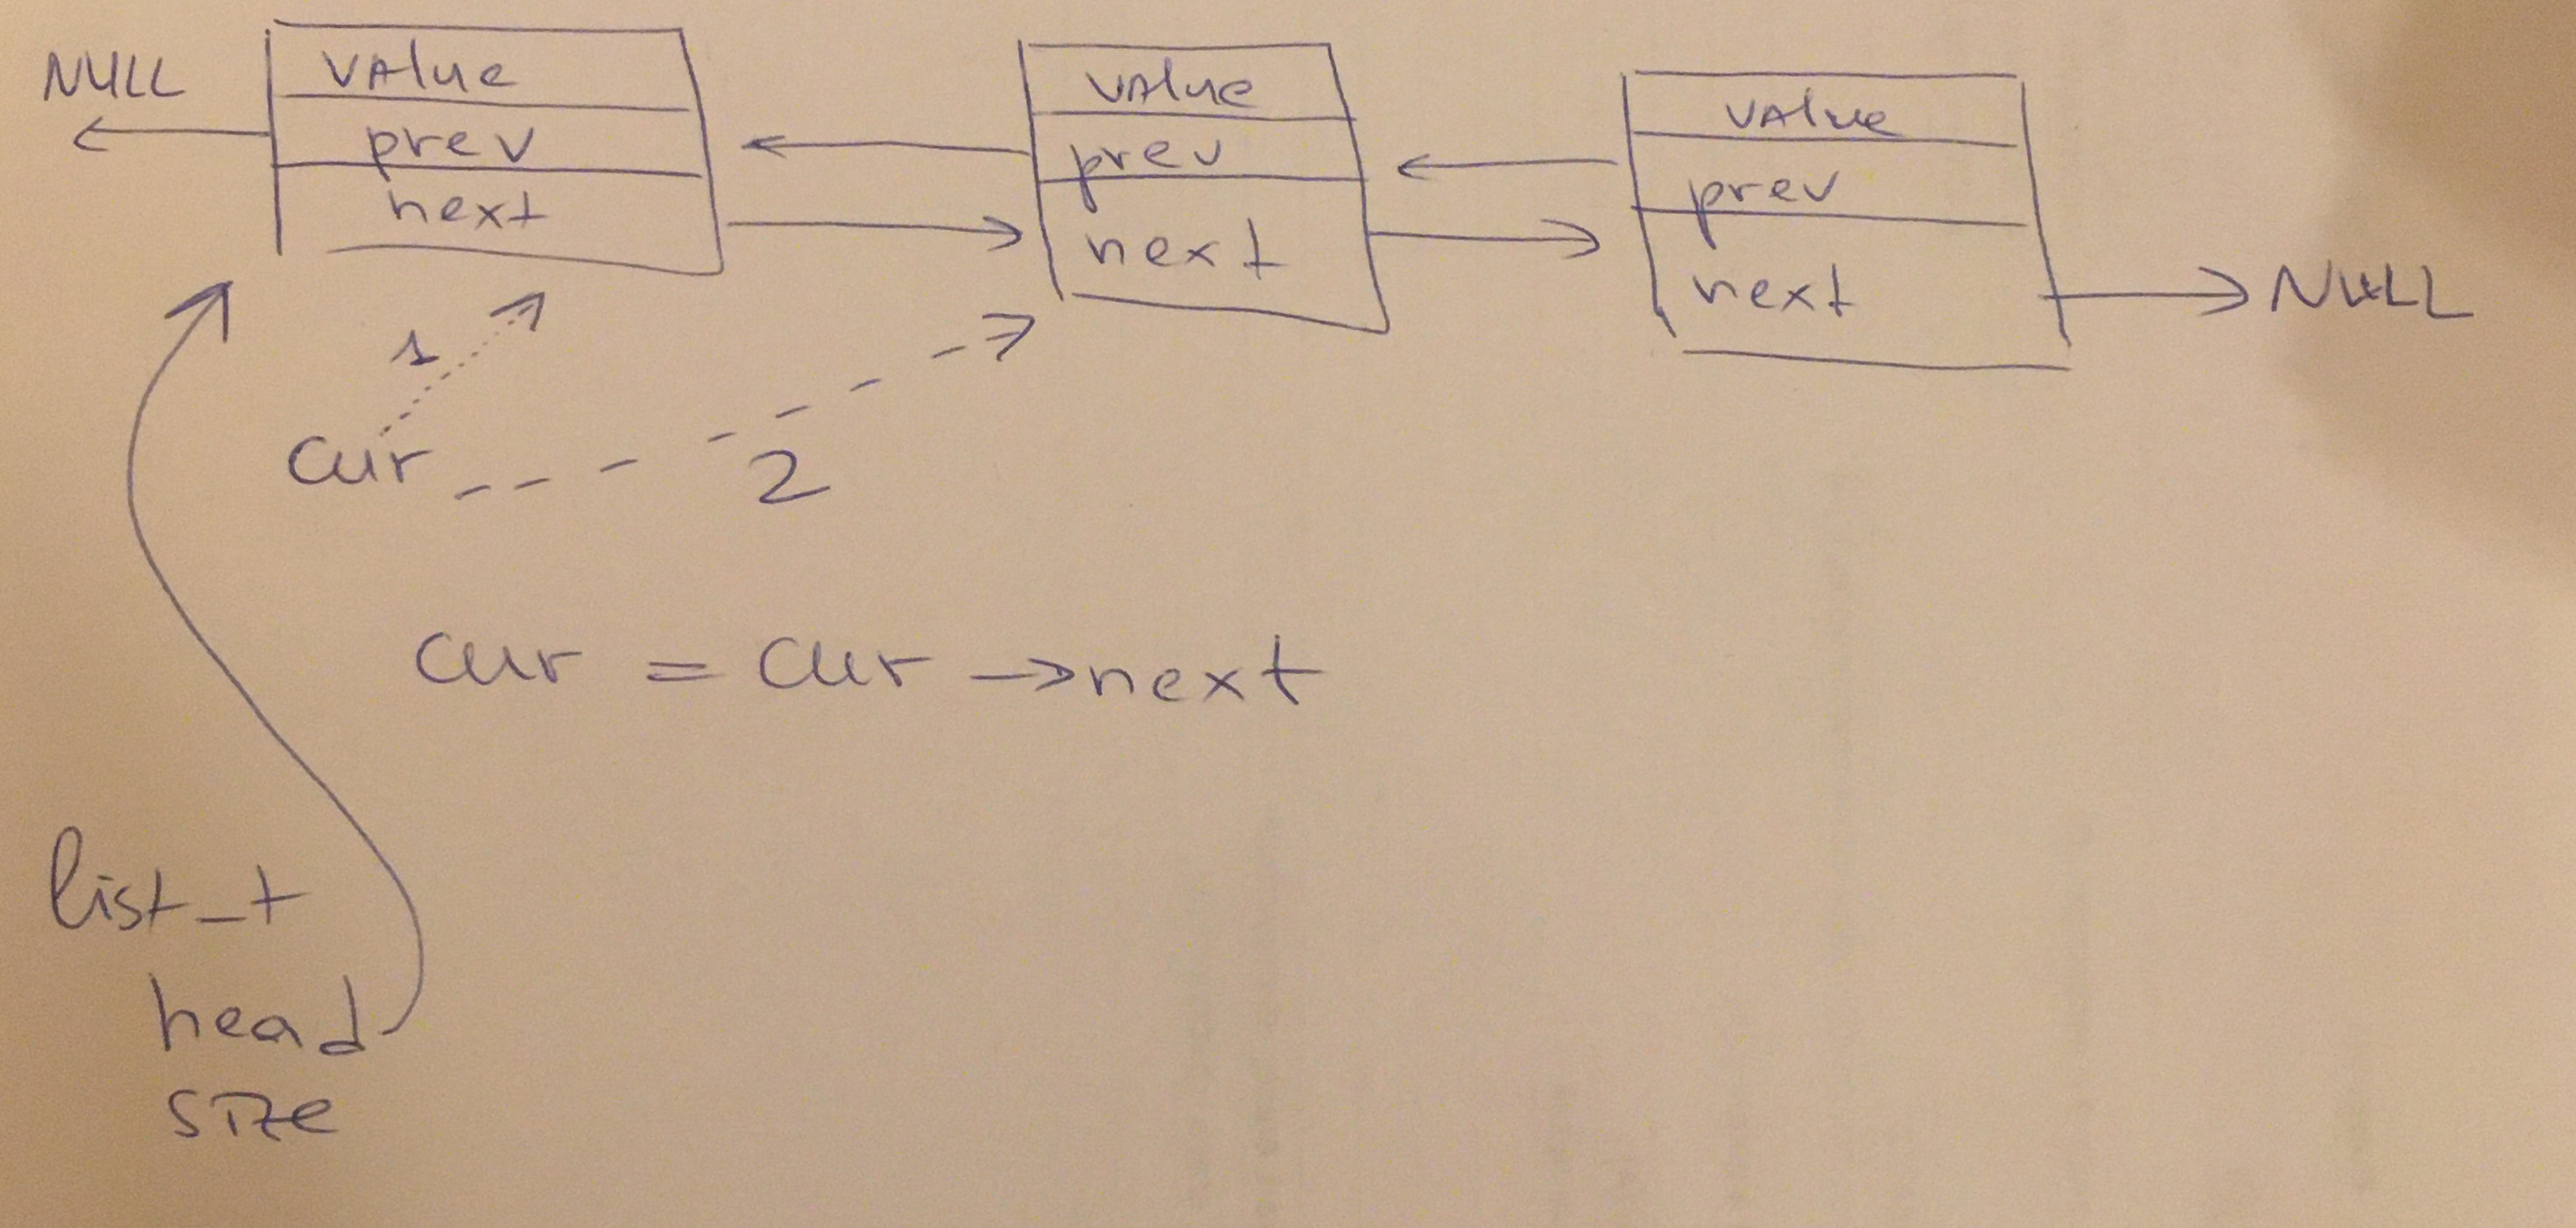
\includegraphics[scale=0.1]{list_iterate}
\end{frame}

\end{document}




